\documentclass[1p]{elsarticle_modified}
%\bibliographystyle{elsarticle-num}

%\usepackage[colorlinks]{hyperref}
%\usepackage{abbrmath_seonhwa} %\Abb, \Ascr, \Acal ,\Abf, \Afrak
\usepackage{amsfonts}
\usepackage{amssymb}
\usepackage{amsmath}
\usepackage{amsthm}
\usepackage{scalefnt}
\usepackage{amsbsy}
\usepackage{kotex}
\usepackage{caption}
\usepackage{subfig}
\usepackage{color}
\usepackage{graphicx}
\usepackage{xcolor} %% white, black, red, green, blue, cyan, magenta, yellow
\usepackage{float}
\usepackage{setspace}
\usepackage{hyperref}

\usepackage{tikz}
\usetikzlibrary{arrows}

\usepackage{multirow}
\usepackage{array} % fixed length table
\usepackage{hhline}

%%%%%%%%%%%%%%%%%%%%%
\makeatletter
\renewcommand*\env@matrix[1][\arraystretch]{%
	\edef\arraystretch{#1}%
	\hskip -\arraycolsep
	\let\@ifnextchar\new@ifnextchar
	\array{*\c@MaxMatrixCols c}}
\makeatother %https://tex.stackexchange.com/questions/14071/how-can-i-increase-the-line-spacing-in-a-matrix
%%%%%%%%%%%%%%%

\usepackage[normalem]{ulem}

\newcommand{\msout}[1]{\ifmmode\text{\sout{\ensuremath{#1}}}\else\sout{#1}\fi}
%SOURCE: \msout is \stkout macro in https://tex.stackexchange.com/questions/20609/strikeout-in-math-mode

\newcommand{\cancel}[1]{
	\ifmmode
	{\color{red}\msout{#1}}
	\else
	{\color{red}\sout{#1}}
	\fi
}

\newcommand{\add}[1]{
	{\color{blue}\uwave{#1}}
}

\newcommand{\replace}[2]{
	\ifmmode
	{\color{red}\msout{#1}}{\color{blue}\uwave{#2}}
	\else
	{\color{red}\sout{#1}}{\color{blue}\uwave{#2}}
	\fi
}

\newcommand{\Sol}{\mathcal{S}} %segment
\newcommand{\D}{D} %diagram
\newcommand{\A}{\mathcal{A}} %arc


%%%%%%%%%%%%%%%%%%%%%%%%%%%%%5 test

\def\sl{\operatorname{\textup{SL}}(2,\Cbb)}
\def\psl{\operatorname{\textup{PSL}}(2,\Cbb)}
\def\quan{\mkern 1mu \triangleright \mkern 1mu}

\theoremstyle{definition}
\newtheorem{thm}{Theorem}[section]
\newtheorem{prop}[thm]{Proposition}
\newtheorem{lem}[thm]{Lemma}
\newtheorem{ques}[thm]{Question}
\newtheorem{cor}[thm]{Corollary}
\newtheorem{defn}[thm]{Definition}
\newtheorem{exam}[thm]{Example}
\newtheorem{rmk}[thm]{Remark}
\newtheorem{alg}[thm]{Algorithm}

\newcommand{\I}{\sqrt{-1}}
\begin{document}

%\begin{frontmatter}
%
%\title{Boundary parabolic representations of knots up to 8 crossings}
%
%%% Group authors per affiliation:
%\author{Yunhi Cho} 
%\address{Department of Mathematics, University of Seoul, Seoul, Korea}
%\ead{yhcho@uos.ac.kr}
%
%
%\author{Seonhwa Kim} %\fnref{s_kim}}
%\address{Center for Geometry and Physics, Institute for Basic Science, Pohang, 37673, Korea}
%\ead{ryeona17@ibs.re.kr}
%
%\author{Hyuk Kim}
%\address{Department of Mathematical Sciences, Seoul National University, Seoul 08826, Korea}
%\ead{hyukkim@snu.ac.kr}
%
%\author{Seokbeom Yoon}
%\address{Department of Mathematical Sciences, Seoul National University, Seoul, 08826,  Korea}
%\ead{sbyoon15@snu.ac.kr}
%
%\begin{abstract}
%We find all boundary parabolic representation of knots up to 8 crossings.
%
%\end{abstract}
%\begin{keyword}
%    \MSC[2010] 57M25 
%\end{keyword}
%
%\end{frontmatter}

%\linenumbers
%\tableofcontents
%
\newcommand\colored[1]{\textcolor{white}{\rule[-0.35ex]{0.8em}{1.4ex}}\kern-0.8em\color{red} #1}%
%\newcommand\colored[1]{\textcolor{white}{ #1}\kern-2.17ex	\textcolor{white}{ #1}\kern-1.81ex	\textcolor{white}{ #1}\kern-2.15ex\color{red}#1	}

{\Large $\underline{11n_{174}~(K11n_{174})}$}

\setlength{\tabcolsep}{10pt}
\renewcommand{\arraystretch}{1.6}
\vspace{1cm}\begin{tabular}{m{100pt}>{\centering\arraybackslash}m{274pt}}
\multirow{5}{120pt}{
	\centering
	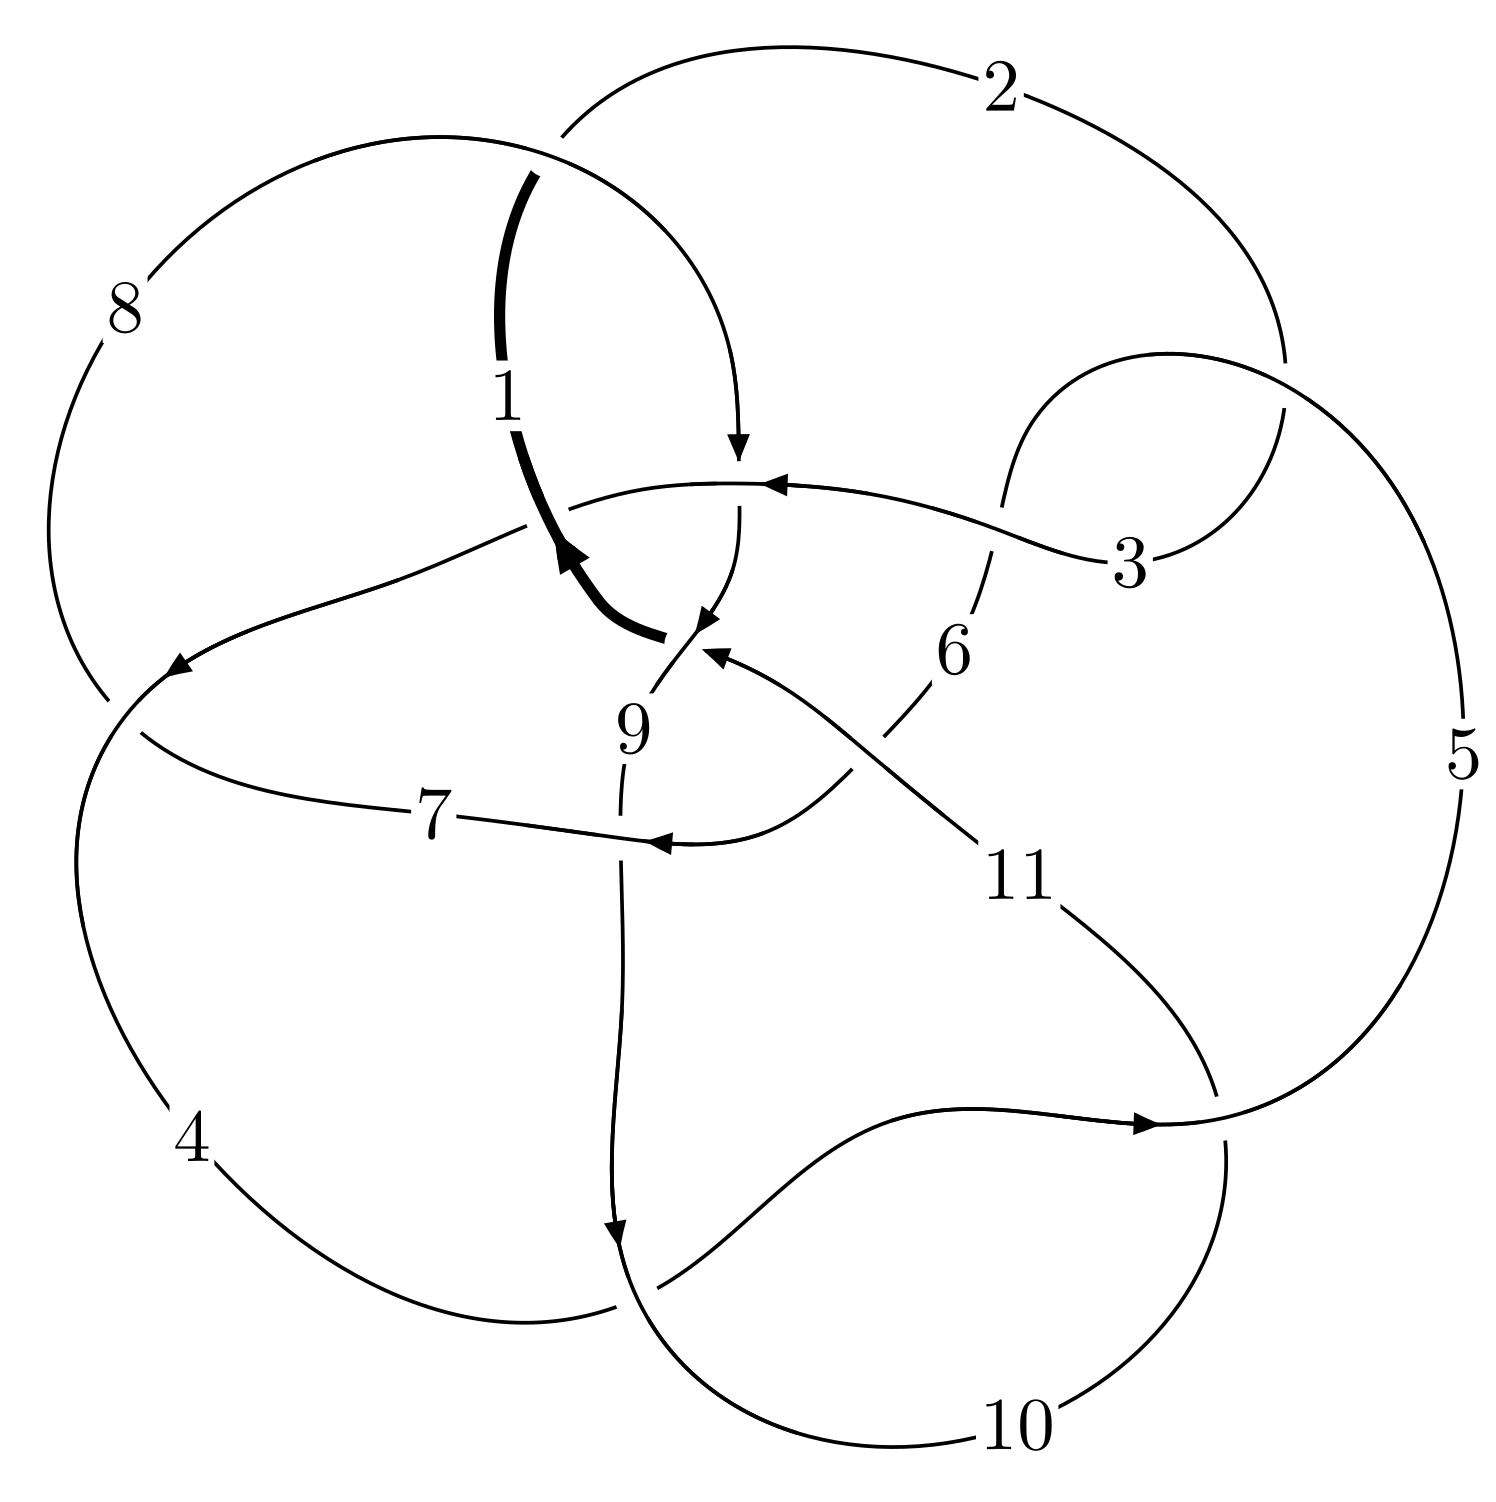
\includegraphics[width=112pt]{../../../GIT/diagram.site/Diagrams/png/790_11n_174.png}\\
\ \ \ A knot diagram\footnotemark}&
\allowdisplaybreaks
\textbf{Linearized knot diagam} \\
\cline{2-2}
 &
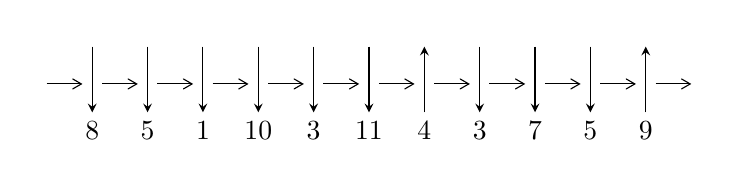
\begin{tikzpicture}[x=20pt, y=17pt]
	% nodes
	\node (C0) at (0, 0) {};
	\node (C1) at (1, 0) {};
	\node (C1U) at (1, +1) {};
	\node (C1D) at (1, -1) {8};

	\node (C2) at (2, 0) {};
	\node (C2U) at (2, +1) {};
	\node (C2D) at (2, -1) {5};

	\node (C3) at (3, 0) {};
	\node (C3U) at (3, +1) {};
	\node (C3D) at (3, -1) {1};

	\node (C4) at (4, 0) {};
	\node (C4U) at (4, +1) {};
	\node (C4D) at (4, -1) {10};

	\node (C5) at (5, 0) {};
	\node (C5U) at (5, +1) {};
	\node (C5D) at (5, -1) {3};

	\node (C6) at (6, 0) {};
	\node (C6U) at (6, +1) {};
	\node (C6D) at (6, -1) {11};

	\node (C7) at (7, 0) {};
	\node (C7U) at (7, +1) {};
	\node (C7D) at (7, -1) {4};

	\node (C8) at (8, 0) {};
	\node (C8U) at (8, +1) {};
	\node (C8D) at (8, -1) {3};

	\node (C9) at (9, 0) {};
	\node (C9U) at (9, +1) {};
	\node (C9D) at (9, -1) {7};

	\node (C10) at (10, 0) {};
	\node (C10U) at (10, +1) {};
	\node (C10D) at (10, -1) {5};

	\node (C11) at (11, 0) {};
	\node (C11U) at (11, +1) {};
	\node (C11D) at (11, -1) {9};
	\node (C12) at (12, 0) {};

	% arrows
	\draw[->,>={angle 60}]
	(C0) edge (C1) (C1) edge (C2) (C2) edge (C3) (C3) edge (C4) (C4) edge (C5) (C5) edge (C6) (C6) edge (C7) (C7) edge (C8) (C8) edge (C9) (C9) edge (C10) (C10) edge (C11) (C11) edge (C12) ;	\draw[->,>=stealth]
	(C1U) edge (C1D) (C2U) edge (C2D) (C3U) edge (C3D) (C4U) edge (C4D) (C5U) edge (C5D) (C6U) edge (C6D) (C7D) edge (C7U) (C8U) edge (C8D) (C9U) edge (C9D) (C10U) edge (C10D) (C11D) edge (C11U) ;
	\end{tikzpicture} \\
\hhline{~~} \\& 
\textbf{Solving Sequence} \\ \cline{2-2} 
 &
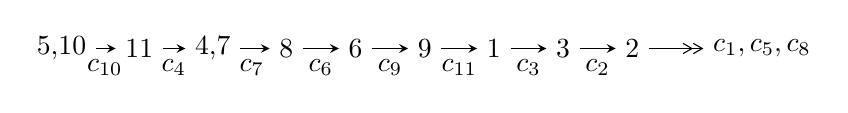
\begin{tikzpicture}[x=25pt, y=7pt]
	% node
	\node (A0) at (-1/8, 0) {5,10};
	\node (A1) at (1, 0) {11};
	\node (A2) at (33/16, 0) {4,7};
	\node (A3) at (25/8, 0) {8};
	\node (A4) at (33/8, 0) {6};
	\node (A5) at (41/8, 0) {9};
	\node (A6) at (49/8, 0) {1};
	\node (A7) at (57/8, 0) {3};
	\node (A8) at (65/8, 0) {2};
	\node (C1) at (1/2, -1) {$c_{10}$};
	\node (C2) at (3/2, -1) {$c_{4}$};
	\node (C3) at (21/8, -1) {$c_{7}$};
	\node (C4) at (29/8, -1) {$c_{6}$};
	\node (C5) at (37/8, -1) {$c_{9}$};
	\node (C6) at (45/8, -1) {$c_{11}$};
	\node (C7) at (53/8, -1) {$c_{3}$};
	\node (C8) at (61/8, -1) {$c_{2}$};
	\node (A9) at (10, 0) {$c_{1},c_{5},c_{8}$};

	% edge
	\draw[->,>=stealth]	
	(A0) edge (A1) (A1) edge (A2) (A2) edge (A3) (A3) edge (A4) (A4) edge (A5) (A5) edge (A6) (A6) edge (A7) (A7) edge (A8) ;
	\draw[->>,>={angle 60}]	
	(A8) edge (A9);
\end{tikzpicture} \\ 

\end{tabular} \\

\footnotetext{
The image of knot diagram is generated by the software ``\textbf{Draw programme}" developed by Andrew Bartholomew(\url{http://www.layer8.co.uk/maths/draw/index.htm\#Running-draw}), where we modified some parts for our purpose(\url{https://github.com/CATsTAILs/LinksPainter}).
}\phantom \\ \newline 
\centering \textbf{Ideals for irreducible components\footnotemark of $X_{\text{par}}$} 
 
\begin{align*}
I^u_{1}&=\langle 
4.62695\times10^{170} u^{68}+1.38051\times10^{170} u^{67}+\cdots+1.85733\times10^{172} b-1.66494\times10^{173},\\
\phantom{I^u_{1}}&\phantom{= \langle  }1.82489\times10^{173} u^{68}+1.22555\times10^{173} u^{67}+\cdots+5.55342\times10^{174} a+8.51358\times10^{174},\\
\phantom{I^u_{1}}&\phantom{= \langle  }u^{69}+u^{68}+\cdots+1241 u-299\rangle \\
I^u_{2}&=\langle 
-169379 u^{20}-231222 u^{19}+\cdots+944459 b+1224184,\\
\phantom{I^u_{2}}&\phantom{= \langle  }-2844830 u^{20}-1101150 u^{19}+\cdots+2833377 a+1086592,\;u^{21}-8 u^{19}+\cdots-5 u+3\rangle \\
\\
\end{align*}
\raggedright * 2 irreducible components of $\dim_{\mathbb{C}}=0$, with total 90 representations.\\
\footnotetext{All coefficients of polynomials are rational numbers. But the coefficients are sometimes approximated in decimal forms when there is not enough margin.}
\newpage
\renewcommand{\arraystretch}{1}
\centering \section*{I. $I^u_{1}= \langle 4.63\times10^{170} u^{68}+1.38\times10^{170} u^{67}+\cdots+1.86\times10^{172} b-1.66\times10^{173},\;1.82\times10^{173} u^{68}+1.23\times10^{173} u^{67}+\cdots+5.55\times10^{174} a+8.51\times10^{174},\;u^{69}+u^{68}+\cdots+1241 u-299 \rangle$}
\flushleft \textbf{(i) Arc colorings}\\
\begin{tabular}{m{7pt} m{180pt} m{7pt} m{180pt} }
\flushright $a_{5}=$&$\begin{pmatrix}0\\u\end{pmatrix}$ \\
\flushright $a_{10}=$&$\begin{pmatrix}1\\0\end{pmatrix}$ \\
\flushright $a_{11}=$&$\begin{pmatrix}1\\u^2\end{pmatrix}$ \\
\flushright $a_{4}=$&$\begin{pmatrix}u\\u\end{pmatrix}$ \\
\flushright $a_{7}=$&$\begin{pmatrix}-0.0328607 u^{68}-0.0220684 u^{67}+\cdots-15.5573 u-1.53303\\-0.0249118 u^{68}-0.00743278 u^{67}+\cdots-37.1756 u+8.96412\end{pmatrix}$ \\
\flushright $a_{8}=$&$\begin{pmatrix}-0.0208503 u^{68}-0.0263337 u^{67}+\cdots-21.4788 u+0.466293\\-0.0129014 u^{68}-0.0116982 u^{67}+\cdots-43.0971 u+10.9635\end{pmatrix}$ \\
\flushright $a_{6}=$&$\begin{pmatrix}-0.0274714 u^{68}-0.0273600 u^{67}+\cdots-29.5143 u+4.20418\\-0.00783605 u^{68}-0.0117040 u^{67}+\cdots-22.3092 u+5.77052\end{pmatrix}$ \\
\flushright $a_{9}=$&$\begin{pmatrix}0.0933496 u^{68}+0.0340529 u^{67}+\cdots+276.120 u-53.7846\\0.0202620 u^{68}-0.00602140 u^{67}+\cdots+101.166 u-24.4436\end{pmatrix}$ \\
\flushright $a_{1}=$&$\begin{pmatrix}-0.126494 u^{68}-0.0228619 u^{67}+\cdots-311.080 u+71.5076\\-0.0303872 u^{68}-0.00849253 u^{67}+\cdots-125.465 u+30.8477\end{pmatrix}$ \\
\flushright $a_{3}=$&$\begin{pmatrix}0.0862458 u^{68}+0.0186000 u^{67}+\cdots+59.5111 u+0.630964\\0.176390 u^{68}+0.0257365 u^{67}+\cdots+229.858 u-37.9084\end{pmatrix}$ \\
\flushright $a_{2}=$&$\begin{pmatrix}0.0862458 u^{68}+0.0186000 u^{67}+\cdots+59.5111 u+0.630964\\0.0922526 u^{68}+0.0308119 u^{67}+\cdots+120.122 u-17.6823\end{pmatrix}$\\ \flushright $a_{2}=$&$\begin{pmatrix}0.0862458 u^{68}+0.0186000 u^{67}+\cdots+59.5111 u+0.630964\\0.0922526 u^{68}+0.0308119 u^{67}+\cdots+120.122 u-17.6823\end{pmatrix}$\\&\end{tabular}
\flushleft \textbf{(ii) Obstruction class $= -1$}\\~\\
\flushleft \textbf{(iii) Cusp Shapes $= 1.16602 u^{68}+0.125596 u^{67}+\cdots+2374.59 u-461.565$}\\~\\
\newpage\renewcommand{\arraystretch}{1}
\flushleft \textbf{(iv) u-Polynomials at the component}\newline \\
\begin{tabular}{m{50pt}|m{274pt}}
Crossings & \hspace{64pt}u-Polynomials at each crossing \\
\hline $$\begin{aligned}c_{1}\end{aligned}$$&$\begin{aligned}
&u^{69}+u^{68}+\cdots-14400 u+2701
\end{aligned}$\\
\hline $$\begin{aligned}c_{2},c_{5}\end{aligned}$$&$\begin{aligned}
&u^{69}+23 u^{67}+\cdots+26 u+1
\end{aligned}$\\
\hline $$\begin{aligned}c_{3}\end{aligned}$$&$\begin{aligned}
&u^{69}-4 u^{68}+\cdots-2 u+1
\end{aligned}$\\
\hline $$\begin{aligned}c_{4},c_{10}\end{aligned}$$&$\begin{aligned}
&u^{69}- u^{68}+\cdots+1241 u+299
\end{aligned}$\\
\hline $$\begin{aligned}c_{6}\end{aligned}$$&$\begin{aligned}
&u^{69}+5 u^{68}+\cdots+41005 u-959
\end{aligned}$\\
\hline $$\begin{aligned}c_{7}\end{aligned}$$&$\begin{aligned}
&u^{69}-3 u^{68}+\cdots-1626 u-131
\end{aligned}$\\
\hline $$\begin{aligned}c_{8}\end{aligned}$$&$\begin{aligned}
&u^{69}- u^{68}+\cdots+26 u-1
\end{aligned}$\\
\hline $$\begin{aligned}c_{9}\end{aligned}$$&$\begin{aligned}
&u^{69}+6 u^{68}+\cdots-431 u-77
\end{aligned}$\\
\hline $$\begin{aligned}c_{11}\end{aligned}$$&$\begin{aligned}
&u^{69}+5 u^{68}+\cdots-144 u+13
\end{aligned}$\\
\hline
\end{tabular}\\~\\
\newpage\renewcommand{\arraystretch}{1}
\flushleft \textbf{(v) Riley Polynomials at the component}\newline \\
\begin{tabular}{m{50pt}|m{274pt}}
Crossings & \hspace{64pt}Riley Polynomials at each crossing \\
\hline $$\begin{aligned}c_{1}\end{aligned}$$&$\begin{aligned}
&y^{69}+y^{68}+\cdots+37585944 y-7295401
\end{aligned}$\\
\hline $$\begin{aligned}c_{2},c_{5}\end{aligned}$$&$\begin{aligned}
&y^{69}+46 y^{68}+\cdots+142 y-1
\end{aligned}$\\
\hline $$\begin{aligned}c_{3}\end{aligned}$$&$\begin{aligned}
&y^{69}-16 y^{68}+\cdots-92 y-1
\end{aligned}$\\
\hline $$\begin{aligned}c_{4},c_{10}\end{aligned}$$&$\begin{aligned}
&y^{69}-39 y^{68}+\cdots+2462795 y-89401
\end{aligned}$\\
\hline $$\begin{aligned}c_{6}\end{aligned}$$&$\begin{aligned}
&y^{69}+5 y^{68}+\cdots+1401617939 y-919681
\end{aligned}$\\
\hline $$\begin{aligned}c_{7}\end{aligned}$$&$\begin{aligned}
&y^{69}+5 y^{68}+\cdots+3046570 y-17161
\end{aligned}$\\
\hline $$\begin{aligned}c_{8}\end{aligned}$$&$\begin{aligned}
&y^{69}+7 y^{68}+\cdots+6292 y-1
\end{aligned}$\\
\hline $$\begin{aligned}c_{9}\end{aligned}$$&$\begin{aligned}
&y^{69}-28 y^{68}+\cdots+272925 y-5929
\end{aligned}$\\
\hline $$\begin{aligned}c_{11}\end{aligned}$$&$\begin{aligned}
&y^{69}-9 y^{68}+\cdots+42316 y-169
\end{aligned}$\\
\hline
\end{tabular}\\~\\
\newpage\flushleft \textbf{(vi) Complex Volumes and Cusp Shapes}
$$\begin{array}{c|c|c}  
\text{Solutions to }I^u_{1}& \I (\text{vol} + \sqrt{-1}CS) & \text{Cusp shape}\\
 \hline 
\begin{aligned}
u &= \phantom{-}0.646999 + 0.771417 I \\
a &= -0.211192 - 0.326936 I \\
b &= \phantom{-}0.896559 - 0.908886 I\end{aligned}
 & \phantom{-}0.416185 + 1.079370 I & \phantom{-0.000000 } 0 \\ \hline\begin{aligned}
u &= \phantom{-}0.646999 - 0.771417 I \\
a &= -0.211192 + 0.326936 I \\
b &= \phantom{-}0.896559 + 0.908886 I\end{aligned}
 & \phantom{-}0.416185 - 1.079370 I & \phantom{-0.000000 } 0 \\ \hline\begin{aligned}
u &= -0.983915 + 0.214466 I \\
a &= \phantom{-}1.212160 + 0.288286 I \\
b &= \phantom{-}1.085450 - 0.882631 I\end{aligned}
 & -4.34006 + 3.63990 I & \phantom{-0.000000 } 0 \\ \hline\begin{aligned}
u &= -0.983915 - 0.214466 I \\
a &= \phantom{-}1.212160 - 0.288286 I \\
b &= \phantom{-}1.085450 + 0.882631 I\end{aligned}
 & -4.34006 - 3.63990 I & \phantom{-0.000000 } 0 \\ \hline\begin{aligned}
u &= -0.989342\phantom{ +0.000000I} \\
a &= \phantom{-}2.42880\phantom{ +0.000000I} \\
b &= \phantom{-}2.35178\phantom{ +0.000000I}\end{aligned}
 & -7.69036\phantom{ +0.000000I} & -12.4710\phantom{ +0.000000I} \\ \hline\begin{aligned}
u &= \phantom{-}0.544955 + 0.860146 I \\
a &= -0.349532 + 0.618138 I \\
b &= -0.949040 + 0.622220 I\end{aligned}
 & -1.48384 + 3.15855 I & \phantom{-0.000000 } 0 \\ \hline\begin{aligned}
u &= \phantom{-}0.544955 - 0.860146 I \\
a &= -0.349532 - 0.618138 I \\
b &= -0.949040 - 0.622220 I\end{aligned}
 & -1.48384 - 3.15855 I & \phantom{-0.000000 } 0 \\ \hline\begin{aligned}
u &= \phantom{-}0.937671 + 0.242423 I \\
a &= \phantom{-}1.80821 + 0.79221 I \\
b &= \phantom{-}0.998024 - 0.477800 I\end{aligned}
 & \phantom{-}0.065178 - 1.027540 I & \phantom{-0.000000 } 0 \\ \hline\begin{aligned}
u &= \phantom{-}0.937671 - 0.242423 I \\
a &= \phantom{-}1.80821 - 0.79221 I \\
b &= \phantom{-}0.998024 + 0.477800 I\end{aligned}
 & \phantom{-}0.065178 + 1.027540 I & \phantom{-0.000000 } 0 \\ \hline\begin{aligned}
u &= \phantom{-}0.912710 + 0.496042 I \\
a &= \phantom{-}0.030686 + 0.640118 I \\
b &= \phantom{-}0.438358 - 1.147020 I\end{aligned}
 & \phantom{-}3.14658 + 2.19858 I & \phantom{-0.000000 } 0\\
 \hline 
 \end{array}$$\newpage$$\begin{array}{c|c|c}  
\text{Solutions to }I^u_{1}& \I (\text{vol} + \sqrt{-1}CS) & \text{Cusp shape}\\
 \hline 
\begin{aligned}
u &= \phantom{-}0.912710 - 0.496042 I \\
a &= \phantom{-}0.030686 - 0.640118 I \\
b &= \phantom{-}0.438358 + 1.147020 I\end{aligned}
 & \phantom{-}3.14658 - 2.19858 I & \phantom{-0.000000 } 0 \\ \hline\begin{aligned}
u &= -0.879619 + 0.352426 I \\
a &= -0.556829 - 1.277600 I \\
b &= -0.775991 + 0.537886 I\end{aligned}
 & -4.72951 + 5.62545 I & -7.00000 - 8.05479 I \\ \hline\begin{aligned}
u &= -0.879619 - 0.352426 I \\
a &= -0.556829 + 1.277600 I \\
b &= -0.775991 - 0.537886 I\end{aligned}
 & -4.72951 - 5.62545 I & -7.00000 + 8.05479 I \\ \hline\begin{aligned}
u &= -0.992117 + 0.371780 I \\
a &= -0.398508 - 0.958996 I \\
b &= -0.832640 + 0.218514 I\end{aligned}
 & -5.20276 - 2.53834 I & \phantom{-0.000000 } 0 \\ \hline\begin{aligned}
u &= -0.992117 - 0.371780 I \\
a &= -0.398508 + 0.958996 I \\
b &= -0.832640 - 0.218514 I\end{aligned}
 & -5.20276 + 2.53834 I & \phantom{-0.000000 } 0 \\ \hline\begin{aligned}
u &= -0.551335 + 0.759408 I \\
a &= -1.45706 - 0.66527 I \\
b &= -0.848128 + 0.357950 I\end{aligned}
 & \phantom{-}4.60897 + 1.94484 I & -7.00000 - 4.19773 I \\ \hline\begin{aligned}
u &= -0.551335 - 0.759408 I \\
a &= -1.45706 + 0.66527 I \\
b &= -0.848128 - 0.357950 I\end{aligned}
 & \phantom{-}4.60897 - 1.94484 I & -7.00000 + 4.19773 I \\ \hline\begin{aligned}
u &= -0.781416 + 0.747040 I \\
a &= -0.845155 + 0.035539 I \\
b &= \phantom{-}0.117045 - 0.392685 I\end{aligned}
 & \phantom{-}3.15602 + 2.89631 I & \phantom{-0.000000 } 0 \\ \hline\begin{aligned}
u &= -0.781416 - 0.747040 I \\
a &= -0.845155 - 0.035539 I \\
b &= \phantom{-}0.117045 + 0.392685 I\end{aligned}
 & \phantom{-}3.15602 - 2.89631 I & \phantom{-0.000000 } 0 \\ \hline\begin{aligned}
u &= \phantom{-}0.836552 + 0.355471 I \\
a &= \phantom{-}3.41431 + 0.11009 I \\
b &= \phantom{-}0.502414 + 0.462655 I\end{aligned}
 & \phantom{-}3.55336 - 5.75372 I & -7.00000 + 11.54806 I\\
 \hline 
 \end{array}$$\newpage$$\begin{array}{c|c|c}  
\text{Solutions to }I^u_{1}& \I (\text{vol} + \sqrt{-1}CS) & \text{Cusp shape}\\
 \hline 
\begin{aligned}
u &= \phantom{-}0.836552 - 0.355471 I \\
a &= \phantom{-}3.41431 - 0.11009 I \\
b &= \phantom{-}0.502414 - 0.462655 I\end{aligned}
 & \phantom{-}3.55336 + 5.75372 I & -7.00000 - 11.54806 I \\ \hline\begin{aligned}
u &= -0.843450 + 0.242120 I \\
a &= \phantom{-}1.26133 + 1.68155 I \\
b &= \phantom{-}1.057060 + 0.267031 I\end{aligned}
 & -3.83982 - 1.81111 I & -13.9331 + 2.5659 I \\ \hline\begin{aligned}
u &= -0.843450 - 0.242120 I \\
a &= \phantom{-}1.26133 - 1.68155 I \\
b &= \phantom{-}1.057060 - 0.267031 I\end{aligned}
 & -3.83982 + 1.81111 I & -13.9331 - 2.5659 I \\ \hline\begin{aligned}
u &= -0.944665 + 0.609755 I \\
a &= -0.642781 - 0.314129 I \\
b &= -0.493148 - 0.791344 I\end{aligned}
 & \phantom{-}3.48160 + 3.20310 I & \phantom{-0.000000 } 0 \\ \hline\begin{aligned}
u &= -0.944665 - 0.609755 I \\
a &= -0.642781 + 0.314129 I \\
b &= -0.493148 + 0.791344 I\end{aligned}
 & \phantom{-}3.48160 - 3.20310 I & \phantom{-0.000000 } 0 \\ \hline\begin{aligned}
u &= -0.812640\phantom{ +0.000000I} \\
a &= \phantom{-}3.87743\phantom{ +0.000000I} \\
b &= \phantom{-}2.19181\phantom{ +0.000000I}\end{aligned}
 & -6.98195\phantom{ +0.000000I} & -37.6100\phantom{ +0.000000I} \\ \hline\begin{aligned}
u &= -1.083740 + 0.490953 I \\
a &= -0.337664 - 0.729476 I \\
b &= -0.69070 - 1.52502 I\end{aligned}
 & \phantom{-}2.99415 + 8.36107 I & \phantom{-0.000000 } 0 \\ \hline\begin{aligned}
u &= -1.083740 - 0.490953 I \\
a &= -0.337664 + 0.729476 I \\
b &= -0.69070 + 1.52502 I\end{aligned}
 & \phantom{-}2.99415 - 8.36107 I & \phantom{-0.000000 } 0 \\ \hline\begin{aligned}
u &= \phantom{-}1.003500 + 0.664719 I \\
a &= \phantom{-}1.64373 - 0.77917 I \\
b &= \phantom{-}1.29183 + 0.97984 I\end{aligned}
 & -0.66031 - 6.51484 I & \phantom{-0.000000 } 0 \\ \hline\begin{aligned}
u &= \phantom{-}1.003500 - 0.664719 I \\
a &= \phantom{-}1.64373 + 0.77917 I \\
b &= \phantom{-}1.29183 - 0.97984 I\end{aligned}
 & -0.66031 + 6.51484 I & \phantom{-0.000000 } 0\\
 \hline 
 \end{array}$$\newpage$$\begin{array}{c|c|c}  
\text{Solutions to }I^u_{1}& \I (\text{vol} + \sqrt{-1}CS) & \text{Cusp shape}\\
 \hline 
\begin{aligned}
u &= \phantom{-}1.138230 + 0.429957 I \\
a &= -1.47102 + 0.04439 I \\
b &= -0.783779 - 0.565791 I\end{aligned}
 & -0.86519 - 1.56917 I & \phantom{-0.000000 } 0 \\ \hline\begin{aligned}
u &= \phantom{-}1.138230 - 0.429957 I \\
a &= -1.47102 - 0.04439 I \\
b &= -0.783779 + 0.565791 I\end{aligned}
 & -0.86519 + 1.56917 I & \phantom{-0.000000 } 0 \\ \hline\begin{aligned}
u &= \phantom{-}1.073130 + 0.613211 I \\
a &= -1.71878 + 0.44891 I \\
b &= -1.43565 - 0.67603 I\end{aligned}
 & -3.14777 - 8.57745 I & \phantom{-0.000000 } 0 \\ \hline\begin{aligned}
u &= \phantom{-}1.073130 - 0.613211 I \\
a &= -1.71878 - 0.44891 I \\
b &= -1.43565 + 0.67603 I\end{aligned}
 & -3.14777 + 8.57745 I & \phantom{-0.000000 } 0 \\ \hline\begin{aligned}
u &= \phantom{-}1.181450 + 0.456884 I \\
a &= \phantom{-}1.69529 + 0.24281 I \\
b &= \phantom{-}1.38781 + 0.83986 I\end{aligned}
 & -1.06984 - 5.59848 I & \phantom{-0.000000 } 0 \\ \hline\begin{aligned}
u &= \phantom{-}1.181450 - 0.456884 I \\
a &= \phantom{-}1.69529 - 0.24281 I \\
b &= \phantom{-}1.38781 - 0.83986 I\end{aligned}
 & -1.06984 + 5.59848 I & \phantom{-0.000000 } 0 \\ \hline\begin{aligned}
u &= -0.461685 + 0.555961 I \\
a &= -2.67569 - 0.54050 I \\
b &= -0.783354 + 0.742055 I\end{aligned}
 & \phantom{-}4.89807 - 4.12724 I & -4.69782 + 0.44028 I \\ \hline\begin{aligned}
u &= -0.461685 - 0.555961 I \\
a &= -2.67569 + 0.54050 I \\
b &= -0.783354 - 0.742055 I\end{aligned}
 & \phantom{-}4.89807 + 4.12724 I & -4.69782 - 0.44028 I \\ \hline\begin{aligned}
u &= \phantom{-}0.345763 + 0.592216 I \\
a &= -0.397171 - 0.641878 I \\
b &= \phantom{-}0.759436 + 0.517199 I\end{aligned}
 & -0.99239 - 1.75950 I & -5.61831 + 3.16702 I \\ \hline\begin{aligned}
u &= \phantom{-}0.345763 - 0.592216 I \\
a &= -0.397171 + 0.641878 I \\
b &= \phantom{-}0.759436 - 0.517199 I\end{aligned}
 & -0.99239 + 1.75950 I & -5.61831 - 3.16702 I\\
 \hline 
 \end{array}$$\newpage$$\begin{array}{c|c|c}  
\text{Solutions to }I^u_{1}& \I (\text{vol} + \sqrt{-1}CS) & \text{Cusp shape}\\
 \hline 
\begin{aligned}
u &= -1.303150 + 0.255913 I \\
a &= \phantom{-}1.199260 - 0.077483 I \\
b &= \phantom{-}0.695903 - 0.824477 I\end{aligned}
 & -3.03191 + 4.92813 I & \phantom{-0.000000 } 0 \\ \hline\begin{aligned}
u &= -1.303150 - 0.255913 I \\
a &= \phantom{-}1.199260 + 0.077483 I \\
b &= \phantom{-}0.695903 + 0.824477 I\end{aligned}
 & -3.03191 - 4.92813 I & \phantom{-0.000000 } 0 \\ \hline\begin{aligned}
u &= -0.264694 + 1.302280 I \\
a &= -0.276135 - 0.075262 I \\
b &= -0.628096 - 0.543055 I\end{aligned}
 & \phantom{-}5.46533 - 1.95793 I & \phantom{-0.000000 } 0 \\ \hline\begin{aligned}
u &= -0.264694 - 1.302280 I \\
a &= -0.276135 + 0.075262 I \\
b &= -0.628096 + 0.543055 I\end{aligned}
 & \phantom{-}5.46533 + 1.95793 I & \phantom{-0.000000 } 0 \\ \hline\begin{aligned}
u &= -1.34209\phantom{ +0.000000I} \\
a &= \phantom{-}1.52954\phantom{ +0.000000I} \\
b &= \phantom{-}1.24410\phantom{ +0.000000I}\end{aligned}
 & -6.44945\phantom{ +0.000000I} & \phantom{-0.000000 } 0 \\ \hline\begin{aligned}
u &= -0.284379 + 1.314310 I \\
a &= -0.186188 - 0.177334 I \\
b &= -0.982920 - 0.710312 I\end{aligned}
 & \phantom{-}4.22642 - 9.68925 I & \phantom{-0.000000 } 0 \\ \hline\begin{aligned}
u &= -0.284379 - 1.314310 I \\
a &= -0.186188 + 0.177334 I \\
b &= -0.982920 + 0.710312 I\end{aligned}
 & \phantom{-}4.22642 + 9.68925 I & \phantom{-0.000000 } 0 \\ \hline\begin{aligned}
u &= \phantom{-}1.009230 + 0.891812 I \\
a &= \phantom{-}0.469205 - 0.687863 I \\
b &= \phantom{-}1.228300 + 0.212557 I\end{aligned}
 & -0.78649 - 3.40776 I & \phantom{-0.000000 } 0 \\ \hline\begin{aligned}
u &= \phantom{-}1.009230 - 0.891812 I \\
a &= \phantom{-}0.469205 + 0.687863 I \\
b &= \phantom{-}1.228300 - 0.212557 I\end{aligned}
 & -0.78649 + 3.40776 I & \phantom{-0.000000 } 0 \\ \hline\begin{aligned}
u &= \phantom{-}1.386720 + 0.203029 I \\
a &= -1.67954 + 0.82158 I \\
b &= -0.652595 - 0.295438 I\end{aligned}
 & -1.67434 - 4.68821 I & \phantom{-0.000000 } 0\\
 \hline 
 \end{array}$$\newpage$$\begin{array}{c|c|c}  
\text{Solutions to }I^u_{1}& \I (\text{vol} + \sqrt{-1}CS) & \text{Cusp shape}\\
 \hline 
\begin{aligned}
u &= \phantom{-}1.386720 - 0.203029 I \\
a &= -1.67954 - 0.82158 I \\
b &= -0.652595 + 0.295438 I\end{aligned}
 & -1.67434 + 4.68821 I & \phantom{-0.000000 } 0 \\ \hline\begin{aligned}
u &= \phantom{-}0.263199 + 0.512655 I \\
a &= \phantom{-}0.314251 - 0.278779 I \\
b &= \phantom{-}0.068496 + 0.982153 I\end{aligned}
 & \phantom{-}1.46946 - 2.23986 I & -4.09553 + 5.07809 I \\ \hline\begin{aligned}
u &= \phantom{-}0.263199 - 0.512655 I \\
a &= \phantom{-}0.314251 + 0.278779 I \\
b &= \phantom{-}0.068496 - 0.982153 I\end{aligned}
 & \phantom{-}1.46946 + 2.23986 I & -4.09553 - 5.07809 I \\ \hline\begin{aligned}
u &= -1.44216 + 0.21699 I \\
a &= \phantom{-}1.45596 - 0.24216 I \\
b &= \phantom{-}1.35370 - 1.16416 I\end{aligned}
 & -6.77713 + 4.78765 I & \phantom{-0.000000 } 0 \\ \hline\begin{aligned}
u &= -1.44216 - 0.21699 I \\
a &= \phantom{-}1.45596 + 0.24216 I \\
b &= \phantom{-}1.35370 + 1.16416 I\end{aligned}
 & -6.77713 - 4.78765 I & \phantom{-0.000000 } 0 \\ \hline\begin{aligned}
u &= -1.34664 + 0.66399 I \\
a &= -1.40126 - 0.24609 I \\
b &= -1.056310 + 0.681780 I\end{aligned}
 & \phantom{-}1.92930 + 8.74493 I & \phantom{-0.000000 } 0 \\ \hline\begin{aligned}
u &= -1.34664 - 0.66399 I \\
a &= -1.40126 + 0.24609 I \\
b &= -1.056310 - 0.681780 I\end{aligned}
 & \phantom{-}1.92930 - 8.74493 I & \phantom{-0.000000 } 0 \\ \hline\begin{aligned}
u &= -1.34848 + 0.70986 I \\
a &= -1.49515 - 0.27888 I \\
b &= -1.30284 + 0.92320 I\end{aligned}
 & \phantom{-}0.8188 + 16.7284 I & \phantom{-0.000000 } 0 \\ \hline\begin{aligned}
u &= -1.34848 - 0.70986 I \\
a &= -1.49515 + 0.27888 I \\
b &= -1.30284 - 0.92320 I\end{aligned}
 & \phantom{-}0.8188 - 16.7284 I & \phantom{-0.000000 } 0 \\ \hline\begin{aligned}
u &= \phantom{-}0.48219 + 1.46172 I \\
a &= -0.058144 - 0.214259 I \\
b &= \phantom{-}0.383661 - 0.274092 I\end{aligned}
 & \phantom{-}4.45642 - 1.12527 I & \phantom{-0.000000 } 0\\
 \hline 
 \end{array}$$\newpage$$\begin{array}{c|c|c}  
\text{Solutions to }I^u_{1}& \I (\text{vol} + \sqrt{-1}CS) & \text{Cusp shape}\\
 \hline 
\begin{aligned}
u &= \phantom{-}0.48219 - 1.46172 I \\
a &= -0.058144 + 0.214259 I \\
b &= \phantom{-}0.383661 + 0.274092 I\end{aligned}
 & \phantom{-}4.45642 + 1.12527 I & \phantom{-0.000000 } 0 \\ \hline\begin{aligned}
u &= \phantom{-}1.35260 + 0.78453 I \\
a &= \phantom{-}0.783396 + 0.049976 I \\
b &= \phantom{-}0.837091 + 0.848083 I\end{aligned}
 & \phantom{-}1.30082 - 6.59534 I & \phantom{-0.000000 } 0 \\ \hline\begin{aligned}
u &= \phantom{-}1.35260 - 0.78453 I \\
a &= \phantom{-}0.783396 - 0.049976 I \\
b &= \phantom{-}0.837091 - 0.848083 I\end{aligned}
 & \phantom{-}1.30082 + 6.59534 I & \phantom{-0.000000 } 0 \\ \hline\begin{aligned}
u &= \phantom{-}0.407799 + 0.154731 I \\
a &= \phantom{-}1.14417 - 1.09443 I \\
b &= \phantom{-}0.473737 - 1.265520 I\end{aligned}
 & \phantom{-}1.79868 + 2.32213 I & -6.69752 - 8.58341 I \\ \hline\begin{aligned}
u &= \phantom{-}0.407799 - 0.154731 I \\
a &= \phantom{-}1.14417 + 1.09443 I \\
b &= \phantom{-}0.473737 + 1.265520 I\end{aligned}
 & \phantom{-}1.79868 - 2.32213 I & -6.69752 + 8.58341 I \\ \hline\begin{aligned}
u &= \phantom{-}0.419858\phantom{ +0.000000I} \\
a &= -0.693573\phantom{ +0.000000I} \\
b &= \phantom{-}0.163880\phantom{ +0.000000I}\end{aligned}
 & -0.763533\phantom{ +0.000000I} & -13.2570\phantom{ +0.000000I} \\ \hline\begin{aligned}
u &= -1.68905\phantom{ +0.000000I} \\
a &= -1.34682\phantom{ +0.000000I} \\
b &= -0.835443\phantom{ +0.000000I}\end{aligned}
 & -10.1736\phantom{ +0.000000I} & \phantom{-0.000000 } 0 \\ \hline\begin{aligned}
u &= \phantom{-}1.69539 + 0.17399 I \\
a &= -0.834045 + 0.259613 I \\
b &= -0.917744 + 0.009907 I\end{aligned}
 & -3.02414 + 3.47680 I & \phantom{-0.000000 } 0 \\ \hline\begin{aligned}
u &= \phantom{-}1.69539 - 0.17399 I \\
a &= -0.834045 - 0.259613 I \\
b &= -0.917744 - 0.009907 I\end{aligned}
 & -3.02414 - 3.47680 I & \phantom{-0.000000 } 0\\
 \hline 
 \end{array}$$\newpage\newpage\renewcommand{\arraystretch}{1}
\centering \section*{II. $I^u_{2}= \langle -1.69\times10^{5} u^{20}-2.31\times10^{5} u^{19}+\cdots+9.44\times10^{5} b+1.22\times10^{6},\;-2.84\times10^{6} u^{20}-1.10\times10^{6} u^{19}+\cdots+2.83\times10^{6} a+1.09\times10^{6},\;u^{21}-8 u^{19}+\cdots-5 u+3 \rangle$}
\flushleft \textbf{(i) Arc colorings}\\
\begin{tabular}{m{7pt} m{180pt} m{7pt} m{180pt} }
\flushright $a_{5}=$&$\begin{pmatrix}0\\u\end{pmatrix}$ \\
\flushright $a_{10}=$&$\begin{pmatrix}1\\0\end{pmatrix}$ \\
\flushright $a_{11}=$&$\begin{pmatrix}1\\u^2\end{pmatrix}$ \\
\flushright $a_{4}=$&$\begin{pmatrix}u\\u\end{pmatrix}$ \\
\flushright $a_{7}=$&$\begin{pmatrix}1.00404 u^{20}+0.388635 u^{19}+\cdots+1.07419 u-0.383497\\0.179340 u^{20}+0.244820 u^{19}+\cdots+0.837749 u-1.29617\end{pmatrix}$ \\
\flushright $a_{8}=$&$\begin{pmatrix}0.278065 u^{20}+0.424159 u^{19}+\cdots+2.82922 u+0.0479498\\-0.546638 u^{20}+0.280344 u^{19}+\cdots+2.59278 u-0.864728\end{pmatrix}$ \\
\flushright $a_{6}=$&$\begin{pmatrix}0.393839 u^{20}+0.436626 u^{19}+\cdots+2.98089 u-0.513766\\-0.0848994 u^{20}+0.462763 u^{19}+\cdots+2.90831 u-1.44015\end{pmatrix}$ \\
\flushright $a_{9}=$&$\begin{pmatrix}1.76207 u^{20}+1.35703 u^{19}+\cdots+5.66155 u-7.63449\\0.844115 u^{20}+0.284923 u^{19}+\cdots+1.65062 u-3.63281\end{pmatrix}$ \\
\flushright $a_{1}=$&$\begin{pmatrix}1.02305 u^{20}+0.397755 u^{19}+\cdots-3.35591 u-0.933981\\1.06778 u^{20}+0.930275 u^{19}+\cdots-1.21589 u-1.92881\end{pmatrix}$ \\
\flushright $a_{3}=$&$\begin{pmatrix}0.111242 u^{20}-0.225450 u^{19}+\cdots-1.70101 u+1.47329\\-0.986755 u^{20}+0.623445 u^{19}+\cdots+3.11692 u+0.482363\end{pmatrix}$ \\
\flushright $a_{2}=$&$\begin{pmatrix}0.111242 u^{20}-0.225450 u^{19}+\cdots-1.70101 u+1.47329\\-0.821127 u^{20}+0.800904 u^{19}+\cdots+4.57789 u-0.193986\end{pmatrix}$\\ \flushright $a_{2}=$&$\begin{pmatrix}0.111242 u^{20}-0.225450 u^{19}+\cdots-1.70101 u+1.47329\\-0.821127 u^{20}+0.800904 u^{19}+\cdots+4.57789 u-0.193986\end{pmatrix}$\\&\end{tabular}
\flushleft \textbf{(ii) Obstruction class $= 1$}\\~\\
\flushleft \textbf{(iii) Cusp Shapes $= -\frac{6854663}{944459} u^{20}-\frac{94727}{944459} u^{19}+\cdots+\frac{15667372}{944459} u-\frac{1422408}{944459}$}\\~\\
\newpage\renewcommand{\arraystretch}{1}
\flushleft \textbf{(iv) u-Polynomials at the component}\newline \\
\begin{tabular}{m{50pt}|m{274pt}}
Crossings & \hspace{64pt}u-Polynomials at each crossing \\
\hline $$\begin{aligned}c_{1}\end{aligned}$$&$\begin{aligned}
&u^{21}-6 u^{19}+\cdots+2 u+3
\end{aligned}$\\
\hline $$\begin{aligned}c_{2}\end{aligned}$$&$\begin{aligned}
&u^{21}- u^{20}+\cdots-2 u-1
\end{aligned}$\\
\hline $$\begin{aligned}c_{3}\end{aligned}$$&$\begin{aligned}
&u^{21}+7 u^{20}+\cdots+6 u+1
\end{aligned}$\\
\hline $$\begin{aligned}c_{4}\end{aligned}$$&$\begin{aligned}
&u^{21}-8 u^{19}+\cdots-5 u-3
\end{aligned}$\\
\hline $$\begin{aligned}c_{5}\end{aligned}$$&$\begin{aligned}
&u^{21}+u^{20}+\cdots-2 u+1
\end{aligned}$\\
\hline $$\begin{aligned}c_{6}\end{aligned}$$&$\begin{aligned}
&u^{21}+4 u^{20}+\cdots+97 u+7
\end{aligned}$\\
\hline $$\begin{aligned}c_{7}\end{aligned}$$&$\begin{aligned}
&u^{21}-8 u^{18}+\cdots-26 u-1
\end{aligned}$\\
\hline $$\begin{aligned}c_{8}\end{aligned}$$&$\begin{aligned}
&u^{21}-5 u^{19}+\cdots-4 u-1
\end{aligned}$\\
\hline $$\begin{aligned}c_{9}\end{aligned}$$&$\begin{aligned}
&u^{21}+11 u^{20}+\cdots+9 u+1
\end{aligned}$\\
\hline $$\begin{aligned}c_{10}\end{aligned}$$&$\begin{aligned}
&u^{21}-8 u^{19}+\cdots-5 u+3
\end{aligned}$\\
\hline $$\begin{aligned}c_{11}\end{aligned}$$&$\begin{aligned}
&u^{21}-2 u^{20}+\cdots-4 u-1
\end{aligned}$\\
\hline
\end{tabular}\\~\\
\newpage\renewcommand{\arraystretch}{1}
\flushleft \textbf{(v) Riley Polynomials at the component}\newline \\
\begin{tabular}{m{50pt}|m{274pt}}
Crossings & \hspace{64pt}Riley Polynomials at each crossing \\
\hline $$\begin{aligned}c_{1}\end{aligned}$$&$\begin{aligned}
&y^{21}-12 y^{20}+\cdots+64 y-9
\end{aligned}$\\
\hline $$\begin{aligned}c_{2},c_{5}\end{aligned}$$&$\begin{aligned}
&y^{21}+5 y^{20}+\cdots+14 y-1
\end{aligned}$\\
\hline $$\begin{aligned}c_{3}\end{aligned}$$&$\begin{aligned}
&y^{21}-9 y^{20}+\cdots-16 y^2-1
\end{aligned}$\\
\hline $$\begin{aligned}c_{4},c_{10}\end{aligned}$$&$\begin{aligned}
&y^{21}-16 y^{20}+\cdots+55 y-9
\end{aligned}$\\
\hline $$\begin{aligned}c_{6}\end{aligned}$$&$\begin{aligned}
&y^{21}-16 y^{20}+\cdots+11327 y-49
\end{aligned}$\\
\hline $$\begin{aligned}c_{7}\end{aligned}$$&$\begin{aligned}
&y^{21}-6 y^{19}+\cdots+666 y-1
\end{aligned}$\\
\hline $$\begin{aligned}c_{8}\end{aligned}$$&$\begin{aligned}
&y^{21}-10 y^{20}+\cdots+12 y-1
\end{aligned}$\\
\hline $$\begin{aligned}c_{9}\end{aligned}$$&$\begin{aligned}
&y^{21}-13 y^{20}+\cdots+9 y-1
\end{aligned}$\\
\hline $$\begin{aligned}c_{11}\end{aligned}$$&$\begin{aligned}
&y^{21}-2 y^{20}+\cdots+24 y-1
\end{aligned}$\\
\hline
\end{tabular}\\~\\
\newpage\flushleft \textbf{(vi) Complex Volumes and Cusp Shapes}
$$\begin{array}{c|c|c}  
\text{Solutions to }I^u_{2}& \I (\text{vol} + \sqrt{-1}CS) & \text{Cusp shape}\\
 \hline 
\begin{aligned}
u &= -1.047640 + 0.248949 I \\
a &= \phantom{-}1.11386 + 1.03676 I \\
b &= \phantom{-}0.889867 - 0.517208 I\end{aligned}
 & -5.46548 + 5.39204 I & -17.4584 - 5.1370 I \\ \hline\begin{aligned}
u &= -1.047640 - 0.248949 I \\
a &= \phantom{-}1.11386 - 1.03676 I \\
b &= \phantom{-}0.889867 + 0.517208 I\end{aligned}
 & -5.46548 - 5.39204 I & -17.4584 + 5.1370 I \\ \hline\begin{aligned}
u &= \phantom{-}1.16767\phantom{ +0.000000I} \\
a &= -2.18668\phantom{ +0.000000I} \\
b &= -2.15365\phantom{ +0.000000I}\end{aligned}
 & -8.35390\phantom{ +0.000000I} & -22.8760\phantom{ +0.000000I} \\ \hline\begin{aligned}
u &= -0.679857 + 0.446838 I \\
a &= -0.127896 - 0.264606 I \\
b &= -0.613519 - 1.245460 I\end{aligned}
 & \phantom{-}1.77824 - 1.61097 I & -7.53353 - 1.62371 I \\ \hline\begin{aligned}
u &= -0.679857 - 0.446838 I \\
a &= -0.127896 + 0.264606 I \\
b &= -0.613519 + 1.245460 I\end{aligned}
 & \phantom{-}1.77824 + 1.61097 I & -7.53353 + 1.62371 I \\ \hline\begin{aligned}
u &= -1.173280 + 0.260964 I \\
a &= \phantom{-}0.881494 + 0.887530 I \\
b &= \phantom{-}0.913294 - 0.046728 I\end{aligned}
 & -5.83828 - 3.07420 I & -16.8807 + 4.9165 I \\ \hline\begin{aligned}
u &= -1.173280 - 0.260964 I \\
a &= \phantom{-}0.881494 - 0.887530 I \\
b &= \phantom{-}0.913294 + 0.046728 I\end{aligned}
 & -5.83828 + 3.07420 I & -16.8807 - 4.9165 I \\ \hline\begin{aligned}
u &= \phantom{-}0.785925\phantom{ +0.000000I} \\
a &= -3.72133\phantom{ +0.000000I} \\
b &= -2.23310\phantom{ +0.000000I}\end{aligned}
 & -6.81637\phantom{ +0.000000I} & \phantom{-}11.9480\phantom{ +0.000000I} \\ \hline\begin{aligned}
u &= -1.120180 + 0.600951 I \\
a &= -1.47135 - 0.18734 I \\
b &= -1.13102 + 0.89771 I\end{aligned}
 & \phantom{-}0.00904 + 5.86285 I & -6.73177 - 5.24479 I \\ \hline\begin{aligned}
u &= -1.120180 - 0.600951 I \\
a &= -1.47135 + 0.18734 I \\
b &= -1.13102 - 0.89771 I\end{aligned}
 & \phantom{-}0.00904 - 5.86285 I & -6.73177 + 5.24479 I\\
 \hline 
 \end{array}$$\newpage$$\begin{array}{c|c|c}  
\text{Solutions to }I^u_{2}& \I (\text{vol} + \sqrt{-1}CS) & \text{Cusp shape}\\
 \hline 
\begin{aligned}
u &= \phantom{-}0.560710 + 0.288461 I \\
a &= \phantom{-}3.24760 - 1.40038 I \\
b &= \phantom{-}0.114885 - 0.587959 I\end{aligned}
 & \phantom{-}3.70067 - 5.02391 I & -6.64273 + 2.70695 I \\ \hline\begin{aligned}
u &= \phantom{-}0.560710 - 0.288461 I \\
a &= \phantom{-}3.24760 + 1.40038 I \\
b &= \phantom{-}0.114885 + 0.587959 I\end{aligned}
 & \phantom{-}3.70067 + 5.02391 I & -6.64273 - 2.70695 I \\ \hline\begin{aligned}
u &= \phantom{-}1.40713 + 0.19832 I \\
a &= -1.50239 - 0.29253 I \\
b &= -1.40025 - 1.20102 I\end{aligned}
 & -6.98589 - 4.93986 I & -24.1840 + 13.1442 I \\ \hline\begin{aligned}
u &= \phantom{-}1.40713 - 0.19832 I \\
a &= -1.50239 + 0.29253 I \\
b &= -1.40025 + 1.20102 I\end{aligned}
 & -6.98589 + 4.93986 I & -24.1840 - 13.1442 I \\ \hline\begin{aligned}
u &= \phantom{-}0.27754 + 1.39957 I \\
a &= \phantom{-}0.064235 - 0.253321 I \\
b &= -0.295868 - 0.174182 I\end{aligned}
 & \phantom{-}4.41960 - 1.49996 I & -7.35710 + 9.23152 I \\ \hline\begin{aligned}
u &= \phantom{-}0.27754 - 1.39957 I \\
a &= \phantom{-}0.064235 + 0.253321 I \\
b &= -0.295868 + 0.174182 I\end{aligned}
 & \phantom{-}4.41960 + 1.49996 I & -7.35710 - 9.23152 I \\ \hline\begin{aligned}
u &= \phantom{-}0.181335 + 0.523673 I \\
a &= \phantom{-}0.794687 + 1.024240 I \\
b &= -0.878799 + 0.633409 I\end{aligned}
 & -2.44382 + 2.36069 I & -11.11778 - 3.12439 I \\ \hline\begin{aligned}
u &= \phantom{-}0.181335 - 0.523673 I \\
a &= \phantom{-}0.794687 - 1.024240 I \\
b &= -0.878799 - 0.633409 I\end{aligned}
 & -2.44382 - 2.36069 I & -11.11778 + 3.12439 I \\ \hline\begin{aligned}
u &= \phantom{-}1.45442 + 0.23658 I \\
a &= -1.196910 + 0.367608 I \\
b &= -0.476403 - 0.419593 I\end{aligned}
 & -1.14902 - 4.42293 I & -3.30825 + 2.88214 I \\ \hline\begin{aligned}
u &= \phantom{-}1.45442 - 0.23658 I \\
a &= -1.196910 - 0.367608 I \\
b &= -0.476403 + 0.419593 I\end{aligned}
 & -1.14902 + 4.42293 I & -3.30825 - 2.88214 I\\
 \hline 
 \end{array}$$\newpage$$\begin{array}{c|c|c}  
\text{Solutions to }I^u_{2}& \I (\text{vol} + \sqrt{-1}CS) & \text{Cusp shape}\\
 \hline 
\begin{aligned}
u &= -1.67395\phantom{ +0.000000I} \\
a &= -1.36531\phantom{ +0.000000I} \\
b &= -0.857609\phantom{ +0.000000I}\end{aligned}
 & -10.2279\phantom{ +0.000000I} & -83.6430\phantom{ +0.000000I}\\
 \hline 
 \end{array}$$\newpage
\newpage\renewcommand{\arraystretch}{1}
\centering \section*{ III. u-Polynomials}
\begin{tabular}{m{50pt}|m{274pt}}
Crossings & \hspace{64pt}u-Polynomials at each crossing \\
\hline $$\begin{aligned}c_{1}\end{aligned}$$&$\begin{aligned}
&(u^{21}-6 u^{19}+\cdots+2 u+3)(u^{69}+u^{68}+\cdots-14400 u+2701)
\end{aligned}$\\
\hline $$\begin{aligned}c_{2}\end{aligned}$$&$\begin{aligned}
&(u^{21}- u^{20}+\cdots-2 u-1)(u^{69}+23 u^{67}+\cdots+26 u+1)
\end{aligned}$\\
\hline $$\begin{aligned}c_{3}\end{aligned}$$&$\begin{aligned}
&(u^{21}+7 u^{20}+\cdots+6 u+1)(u^{69}-4 u^{68}+\cdots-2 u+1)
\end{aligned}$\\
\hline $$\begin{aligned}c_{4}\end{aligned}$$&$\begin{aligned}
&(u^{21}-8 u^{19}+\cdots-5 u-3)(u^{69}- u^{68}+\cdots+1241 u+299)
\end{aligned}$\\
\hline $$\begin{aligned}c_{5}\end{aligned}$$&$\begin{aligned}
&(u^{21}+u^{20}+\cdots-2 u+1)(u^{69}+23 u^{67}+\cdots+26 u+1)
\end{aligned}$\\
\hline $$\begin{aligned}c_{6}\end{aligned}$$&$\begin{aligned}
&(u^{21}+4 u^{20}+\cdots+97 u+7)(u^{69}+5 u^{68}+\cdots+41005 u-959)
\end{aligned}$\\
\hline $$\begin{aligned}c_{7}\end{aligned}$$&$\begin{aligned}
&(u^{21}-8 u^{18}+\cdots-26 u-1)(u^{69}-3 u^{68}+\cdots-1626 u-131)
\end{aligned}$\\
\hline $$\begin{aligned}c_{8}\end{aligned}$$&$\begin{aligned}
&(u^{21}-5 u^{19}+\cdots-4 u-1)(u^{69}- u^{68}+\cdots+26 u-1)
\end{aligned}$\\
\hline $$\begin{aligned}c_{9}\end{aligned}$$&$\begin{aligned}
&(u^{21}+11 u^{20}+\cdots+9 u+1)(u^{69}+6 u^{68}+\cdots-431 u-77)
\end{aligned}$\\
\hline $$\begin{aligned}c_{10}\end{aligned}$$&$\begin{aligned}
&(u^{21}-8 u^{19}+\cdots-5 u+3)(u^{69}- u^{68}+\cdots+1241 u+299)
\end{aligned}$\\
\hline $$\begin{aligned}c_{11}\end{aligned}$$&$\begin{aligned}
&(u^{21}-2 u^{20}+\cdots-4 u-1)(u^{69}+5 u^{68}+\cdots-144 u+13)
\end{aligned}$\\
\hline
\end{tabular}\newpage\renewcommand{\arraystretch}{1}
\centering \section*{ IV. Riley Polynomials}
\begin{tabular}{m{50pt}|m{274pt}}
Crossings & \hspace{64pt}Riley Polynomials at each crossing \\
\hline $$\begin{aligned}c_{1}\end{aligned}$$&$\begin{aligned}
&(y^{21}-12 y^{20}+\cdots+64 y-9)\\
&\cdot(y^{69}+y^{68}+\cdots+37585944 y-7295401)
\end{aligned}$\\
\hline $$\begin{aligned}c_{2},c_{5}\end{aligned}$$&$\begin{aligned}
&(y^{21}+5 y^{20}+\cdots+14 y-1)(y^{69}+46 y^{68}+\cdots+142 y-1)
\end{aligned}$\\
\hline $$\begin{aligned}c_{3}\end{aligned}$$&$\begin{aligned}
&(y^{21}-9 y^{20}+\cdots-16 y^2-1)(y^{69}-16 y^{68}+\cdots-92 y-1)
\end{aligned}$\\
\hline $$\begin{aligned}c_{4},c_{10}\end{aligned}$$&$\begin{aligned}
&(y^{21}-16 y^{20}+\cdots+55 y-9)(y^{69}-39 y^{68}+\cdots+2462795 y-89401)
\end{aligned}$\\
\hline $$\begin{aligned}c_{6}\end{aligned}$$&$\begin{aligned}
&(y^{21}-16 y^{20}+\cdots+11327 y-49)\\
&\cdot(y^{69}+5 y^{68}+\cdots+1401617939 y-919681)
\end{aligned}$\\
\hline $$\begin{aligned}c_{7}\end{aligned}$$&$\begin{aligned}
&(y^{21}-6 y^{19}+\cdots+666 y-1)(y^{69}+5 y^{68}+\cdots+3046570 y-17161)
\end{aligned}$\\
\hline $$\begin{aligned}c_{8}\end{aligned}$$&$\begin{aligned}
&(y^{21}-10 y^{20}+\cdots+12 y-1)(y^{69}+7 y^{68}+\cdots+6292 y-1)
\end{aligned}$\\
\hline $$\begin{aligned}c_{9}\end{aligned}$$&$\begin{aligned}
&(y^{21}-13 y^{20}+\cdots+9 y-1)(y^{69}-28 y^{68}+\cdots+272925 y-5929)
\end{aligned}$\\
\hline $$\begin{aligned}c_{11}\end{aligned}$$&$\begin{aligned}
&(y^{21}-2 y^{20}+\cdots+24 y-1)(y^{69}-9 y^{68}+\cdots+42316 y-169)
\end{aligned}$\\
\hline
\end{tabular}
\vskip 2pc
\end{document}